%--------1---------2---------3---------4---------5---------6---------7

%\documentclass[10pt, conference, compsocconf]{IEEEtran}
%\documentclass[10pt,conference,compsocconf]{IEEEtran}
\documentclass[10pt,conference]{IEEEtran} 


%\documentclass[times, 10pt,twocolumn]{article} 
%\usepackage{latex8}
%\usepackage{times}
\usepackage{amsfonts}
\usepackage[latin1]{inputenc}
\usepackage[english]{babel}
\usepackage{listings}
\usepackage{algorithmic}
\usepackage{float}
\usepackage[numbers,sort&compress,square]{natbib}
\usepackage{graphicx}
\usepackage{booktabs}
\usepackage{subfigure}
%\usepackage{hyperref}
\usepackage{color}
\usepackage[usenames,dvipsnames,table]{xcolor}
\usepackage{soul}
\usepackage{xspace}
\usepackage{boxedminipage}
\usepackage{alltt}
\usepackage{multirow}
\usepackage{paralist}
\usepackage{amsmath}
\usepackage{balance}
\definecolor{light-gray}{gray}{0.90}

\floatstyle{ruled}
\newfloat{algorithm}{tbp}{loa}
\floatname{algorithm}{Algorithm}

\newtheorem{definition}{Definition}


 %krams hinter fontadjust ist neu
  \definecolor{lightgrey}{rgb}{0.90,0.90,0.90}
\lstset{escapeinside={(*}{*)}}
  \lstloadlanguages{java}
 \lstdefinelanguage{pseudocode}
  {morekeywords={if, else, initialize, return, for, each, in, global, new}
   }
  \lstset{
    tabsize=2,
    mathescape=true,
    escapeinside={(*}{*)},
    captionpos=t,
    framerule=0pt,
    backgroundcolor=\color{lightgrey},
    basicstyle=\scriptsize\ttfamily,
    keywordstyle=\footnotesize\bfseries,
    numbers=none,
    numberstyle=\tiny,
    numbersep=1pt,
    fontadjust,
    breaklines=true,
    breakatwhitespace=false
  }    
      

% \hypersetup{
% colorlinks=true,
% urlcolor=rltblue,
% linkcolor=rltred,
% citecolor=rltgreen,
% bookmarksnumbered=true,
% pdftitle={EvoSuite at the SBST 2016 Tool Competition},
% pdfauthor={Gordon Fraser and Andrea Arcuri},
% pdfsubject={Test case generation},
% pdfkeywords={Test case generation, unit testing, test
%   oracles, assertions, search based testing}
% }

\definecolor{rltred}{rgb}{0.5,0,0}
\definecolor{rltgreen}{rgb}{0,0.5,0}
\definecolor{rltblue}{rgb}{0,0,0.5}
\definecolor{ScarletRed}{rgb}{0.80,0.00,0.00}



% in draft mode we put \remarks into the margins and do other stuff
% set to \draftfalse for 
\newif\ifdraft
\draftfalse

\ifdraft
	\marginparwidth=1.3cm
	\marginparsep=5pt
	\newcommand\remark[1]{%
		\mymarginpar{\raggedright\hbadness=10000\tiny\it #1\par}}
	% TODO marker
	\newcommand{\TODO}[1]{\sethlcolor{yellow}\textbf{\textcolor{ScarletRed}{\hl{TODO: #1}}}\xspace}
\else
	\newcommand\remark[1]	{}
	\newcommand{\TODO}[1]{}
\fi

\ifdraft
	\overfullrule3pt
\fi    

% We use \FIXME for located problems (``defect'')
\newcommand{\FIXME}[1]{\remark{FIXME: #1}}
\newcommand\parremark[1]	{\par\textbf{REMARK:} #1\par}

\newcommand{\gordon}[1]{\textcolor{blue}{\sf\small\textbf{Gordon:} #1}}
\newcommand{\andrea}[1]{\textcolor{ScarletRed}{\sf\small\textbf{Andrea:} #1}}

% \mathid is used to denote identifiers and slots in formulas
\newcommand{\mathid}[1]{\text{\rmfamily\textit{#1}}}

% But usually, we shall use \|name| instead.
\def\|#1|{\mathid{#1}}

% \codeid is used to denote computer code identifiers
\newcommand{\codeid}[1]{\texttt{#1}}

% But usually, we shall use \<name> instead.
\def\<#1>{\codeid{#1}}

% Our results
\newenvironment{result}%
{\smallskip
\noindent
\let\emph=\textbf
\begin{boxedminipage}{\columnwidth}\begin{center}\em}%
{\end{center}\end{boxedminipage}%
\smallskip
}

\newcommand{\JodaTime}{Joda-Time\xspace}  % That's how they write themselves -- AZ

\newcommand{\EVOSUITE}{\textsc{EvoSuite}\xspace}
\newcommand{\JTEXPERT}{\textsc{jTExpert}\xspace}
\newcommand{\RANDOOP}{\textsc{Randoop}\xspace}
\newcommand{\TT}{\textsc{T3}\xspace}

\newcommand{\MUTEST}{{\sc $\mu$Test}\xspace}
\newcommand{\CS}{{\sc SF100}\xspace}


\DeclareMathSymbol{,}{\mathpunct}{letters}{"3B}
\DeclareMathSymbol{,}{\mathord}{letters}{"3B}
\DeclareMathSymbol{\decimal}{\mathord}{letters}{"3A}
%%%"

\usepackage{siunitx}
\newcommand{\score}{\num{380.57}\xspace}
\newcommand{\cuts}{\num{65}\xspace}
\newcommand{\budgetShort}{\SI{30}{\second}\xspace}
\newcommand{\budgetLong}{\SI{120}{\second}\xspace}
\newcommand{\avgLinesCoverageRatioShort}{\SI[round-mode=figures,round-precision=3]{51.87307894984616}{\percent}\xspace}
\newcommand{\medLinesCoverageRatioShort}{\SI[round-mode=figures,round-precision=3]{46.666668}{\percent}\xspace}
\newcommand{\avgLinesCoverageRatioLong}{\SI[round-mode=figures,round-precision=3]{62.73892781107692}{\percent}\xspace}
\newcommand{\medLinesCoverageRatioLong}{\SI[round-mode=figures,round-precision=3]{71.71428499999999}{\percent}\xspace}
\newcommand{\avgConditionsCoverageRatioShort}{\SI[round-mode=figures,round-precision=3]{46.11903214169231}{\percent}\xspace}
\newcommand{\medConditionsCoverageRatioShort}{\SI[round-mode=figures,round-precision=3]{47.22222}{\percent}\xspace}
\newcommand{\avgConditionsCoverageRatioLong}{\SI[round-mode=figures,round-precision=3]{56.821364993692306}{\percent}\xspace}
\newcommand{\medConditionsCoverageRatioLong}{\SI[round-mode=figures,round-precision=3]{60.000004}{\percent}\xspace}
\newcommand{\avgMutantsCoverageRatioShort}{\SI[round-mode=figures,round-precision=3]{39.44754914507693}{\percent}\xspace}
\newcommand{\medMutantsCoverageRatioShort}{\SI[round-mode=figures,round-precision=3]{20.353981}{\percent}\xspace}
\newcommand{\avgMutantsCoverageRatioLong}{\SI[round-mode=figures,round-precision=3]{34.111612112}{\percent}\xspace}
\newcommand{\medMutantsCoverageRatioLong}{\SI[round-mode=figures,round-precision=3]{0.0}{\percent}\xspace}
\newcommand{\numTestGenFailedShort}{\num{21}\xspace}
\newcommand{\numTestGenFailedLong}{\num{26}\xspace}

%------------------------------------------------------------------------- 
% take the % away on next line to produce the final camera-ready version 
%\pagestyle{empty}

%------------------------------------------------------------------------- 
\begin{document}

% 

%\title{Unit Testing Tool competition: Results for EvoSuite}
\title{\EVOSUITE at the SBST 2022 Tool Competition}
 

\author{%
%
\IEEEauthorblockN{%
Sebastian Schweikl\IEEEauthorrefmark{1},
Gordon Fraser\IEEEauthorrefmark{1}, 
Andrea Arcuri\IEEEauthorrefmark{2},
Jose Campos\IEEEauthorrefmark{3},
and Annibale Panichella\IEEEauthorrefmark{4}%
}
%
\IEEEauthorblockA{\IEEEauthorrefmark{1}University of Passau, Germany\\
\{sebastian.vogl,sebastian.schweikl,gordon.fraser\}@uni-passau.de}
\IEEEauthorblockA{\IEEEauthorrefmark{2}Kristiania University College and Oslo Metropolitan University, Norway\\andrea.arcuri@kristiania.no}
\IEEEauthorblockA{\IEEEauthorrefmark{3}University of Lisbon, Portugal\\jcmcampos@fc.ul.pt}
\IEEEauthorblockA{\IEEEauthorrefmark{4}Delft University of Technology, Netherlands\\A.Panichella@tudelft.nl}%
}

\maketitle
%\thispagestyle{empty}

\begin{abstract}
  \EVOSUITE is a search-based unit test generation tool for Java. This paper summarises the results and experiences of \EVOSUITE's participation at the 10th unit testing competition at SBST 2022, where \EVOSUITE achieved the highest overall score.
\end{abstract}



%------------------------------------------------------------------------- 
\section{Introduction}
%
The annual unit test generation competition aims to drive and evaluate progress
on unit test generation tools. Every year, a benchmark of Java classes is
selected, and different test generation tools are evaluated in terms of the
code coverage and mutation scores they can achieve on these classes. In the
2022 edition of the competition, seven tools were applied on a set of \cuts classes.
Details about the procedure of the competition, the technical framework, and
the benchmark classes can be found in the competition report~\cite{SBST-toolcomp22}.
\EVOSUITE achieved an overall score of \score, which was the highest among the
competing and baseline tools.


%------------------------------------------------------------------------- 
\section{About EvoSuite}


\EVOSUITE~\cite{FrA11c} uses evolutionary search to automatically generate test
suites for Java classes. It takes as input the name of a target class as well
as the classpath describing where the compiled bytecode of the class as well as
its dependencies are located. A basic static analysis extracts information
about the relevant classes as well as their constructors, methods, and fields.
The bytecode is instrumented while classes are loaded, such that \EVOSUITE can
produce execution traces for test executions, and to avoid test flakiness by
replacing non-deterministic calls with deterministic, mocked versions.
\EVOSUITE then applies meta-heuristic search algorithms to automatically
produce a set of JUnit test cases aimed at maximising code coverage.
%Besides the basic command line interface there are also plugins for popular development environments such as IntelliJ, Eclipse, or Maven~\cite{ICST16_Tool}.


Originally, \EVOSUITE was implemented to optimise entire test suites with
respect to their overall code coverage~\cite{GoA_TSE12}. The latest search algorithm, which is now used by default, is the \textit{Dynamic Many-Objective Sorting Algorithm} (DynaMOSA) search algorithm~\cite{dynamosa} which operates at the test case level. 
%
The genetic encoding of test cases in \EVOSUITE consists of variable-length sequences of Java statements (e.g., primitive statements as well as calls on constructors or methods). Standard evolutionary search operators (e.g., selection, crossover, mutation) are adapted for this representation. 
%
\EVOSUITE supports multiple different coverage criteria that can be optimised simultaneously. The core fitness functions in \EVOSUITE are based on traditional heuristics for code coverage, such as the branch distance and the approach level (see~\cite{GoA_TSE12} for more details). Further fitness functions are based on mutation testing~\cite{emse14_mutation} as well as other basic criteria~\cite{rojas2015combining}.


To improve the readability of the generated tests and to avoid test smells~\cite{panichella2020revisiting}, \EVOSUITE applies post-processing once the available search budget has been exhausted~\cite{FrA11c,FrA13a}. In particular, minimisation is used to remove redundant tests and statements, and a minimised set of assertions is added using mutation analysis~\cite{10.1109/TSE.2011.93}. Finally, \EVOSUITE compiles and executes each test individually to avoid compilation errors (which may be the result of bugs in \EVOSUITE) or flakiness caused by non-determinism in the class under test.

%Besides multiple in-depth empirical evaluations of \EVOSUITE with respect to
%code coverage~\cite{fraser2014large,emse_archive,ea_evaluation,dynamosa},
%fault-finding effectiveness~\cite{shamshiri2015automatically,moein2017}, and
%effects on developer productivity~\cite{TOSEM_userstudy,ISSTA15_Study} and
%software maintenance~\cite{ICST2018_Maintenance}, \EVOSUITE has also participated in all prior instances of the unit testing tool competition, usually ranking among the best performing tools.





%------------------------------------------------------------------------- 
\section{Competition Setup}


The most recent version of \EVOSUITE (1.1.0) was used in the competition. As of
this version, the default search algorithm in \EVOSUITE is
DynaMOSA~\cite{dynamosa}. No new features were added in this version, but
support for Java 9+ was added, several bugs were fixed, and a major refactoring
was applied to improve the code quality with respect to the use of Java
generics internally. Several smaller bugfixes were applied in the run-up to the
competition, which are now included in the current development version on
GitHub.

The configuration of \EVOSUITE used in the 2021 competition is identical to the
configuration used in prior years, and largely based on its tuned default
values~\cite{arcuri2013parameter} and default coverage criteria
\cite{rojas2015combining}.
%
Similar to prior competitions, the test minimisation step was omitted as the competition score does not reward test minimality, and the minimisation takes substantial computational effort. Similarly, we included all regression assertions rather than filtering them with mutation analysis to save time. 
%
Same as in previous competitions, we allocated 50\% of
the overall time set by the competition organisers for the search, and
distributed the other 50\% equally to the remaining phases (e.g., assertion generation, compile-check, flakiness-check).



%------------------------------------------------------------------------- 
\section{Results}

\begin{figure}
	\centering
	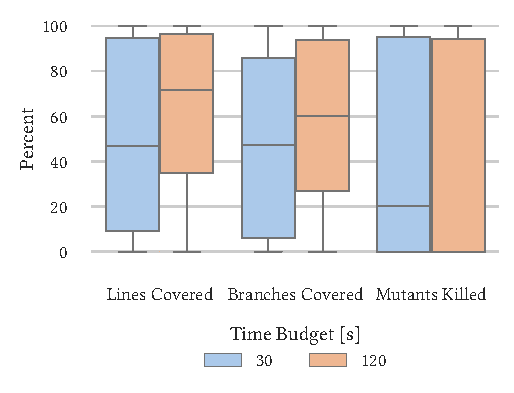
\includegraphics[width=\columnwidth]{data/CoverageBoxV}
	\vspace{-2em}
	\caption{\label{fig:results}Coverage results achieved in the competition.}
	\vspace{-1em}
\end{figure}


With an overall score of \score, \EVOSUITE achieved the highest score of all
tools in the competition. As described in the competition
report~\cite{SBST-toolcomp22}, the score is calculated on the subset of \cuts classes
for which all tools produced tests in some of the runs.
Figure~\ref{fig:results} summarises the results of \EVOSUITE in terms of the
mean coverage for the \cuts classes used in the competition. While the coverage
increased from the \budgetShort to the \budgetLong search budget (mean line
coverage of \avgLinesCoverageRatioShort vs. \avgLinesCoverageRatioLong, respectively),
the additional run of 300 seconds
actually shows a slight decrease (mean line coverage of 73.9\%). The likely
reason for this result is that \EVOSUITE crashed more frequently when given
more time. For example, for 76 runs of \EVOSUITE on the \cuts classes no test
cases were generated. In most cases we found that the JVM process running
\EVOSUITE on the competition machine crashed with an
\texttt{OutOfMemoryException}, which possibly could have been avoided with a
more generous allocation of memory.

The coverage ratios are generally higher than the mutation scores; while this is largely because it is simply more difficult to achieve a high mutation score, the mutation score is also negatively affected by classes with flakiness or failing tests (in which case the mutation score reported is 0\% by definition). Furthermore, in many cases the execution with the PIT mutation tool reported an error during class loading, which may be caused by configuration errors or clashes between \EVOSUITE's and PIT's bytecode instrumentation.


A final observation is that all \cuts Java classes considered in the competition
results were taken from the Guava project, which is notorious for its complex
use of Java Generics---which is a feature \EVOSUITE still struggles to handle
effectively. In particular, in 99 of all runs on the \cuts competition classes
\EVOSUITE did not manage to move beyond the initial generation, which tends to
happen specifically when \EVOSUITE struggles to correctly instantiate complex,
nested generic types. This is currently a focus point of structural
improvements and refactorings in \EVOSUITE's codebase.






%------------------------------------------------------------------------- 
\section{Conclusions}

This paper reports on the participation of the \EVOSUITE test generation tool
in the tenth SBST Java Unit Testing Tool Contest. On average, \EVOSUITE achieved
\avgConditionsCoverageRatioLong branch coverage, \avgLinesCoverageRatioLong line coverage, 
and a mutation score of \avgMutantsCoverageRatioLong, using a
search budget of \budgetLong on the \cuts classes considered for the competition.
Overall, this results in a score of \score, which is the highest score of all
tools in the competition.


To learn more about \EVOSUITE, visit our Web site:
\begin{center}
%\url{http://evosuite.org/}
\texttt{http://www.evosuite.org}
\end{center}


%------------------------------------------------------------------------- 

%\noindent
\textbf{Acknowledgments:} Many thanks to all the contributors to
\EVOSUITE.
This project has been supported by EPSRC project % ``GREATEST'' 
EP/N023978/2.


%------------------------------------------------------------------------- 
%\def\IEEEbibitemsep{5pt plus 1pt}
%\def\IEEEbibitemsep{6pt}
%\clearpage
\bibliographystyle{IEEEtranS}
\bibliography{papers}
\balance

\end{document}


%%% Local Variables:
%%% mode: latex
%%% TeX-master: t
%%% End:
